\documentclass[12pt]{report}
\usepackage[utf8]{inputenc}
\usepackage[T2A]{fontenc}
\usepackage[russian]{babel}

\usepackage{amsmath,amsfonts,amssymb,amsthm,mathtools}
\DeclarePairedDelimiter\abs{\lvert}{\rvert}

\usepackage{pgfplots}
\usepackage{filecontents}
\usepackage{indentfirst}
\usepackage{eucal}
\usepackage{enumitem}
% Для \abs{}
\usepackage{commath}
\usepackage{float}
\frenchspacing

% Для нормальных переносов
\sloppy

\usetikzlibrary{datavisualization}
\usetikzlibrary{datavisualization.formats.functions}

\usepackage[left=2cm,right=2cm, top=2cm,bottom=2cm,bindingoffset=0cm]{geometry}
% Для измененных титулов глав:
\usepackage{titlesec, blindtext, color} % подключаем нужные пакеты
\definecolor{gray75}{gray}{0.75} % определяем цвет
\newcommand{\hsp}{\hspace{20pt}} % длина линии в 20pt
% titleformat определяет стиль
\titleformat{\chapter}[hang]{\Huge\bfseries}{\thechapter\hsp\textcolor{gray75}{|}\hsp}{0pt}{\Huge\bfseries}

% plot
\usepackage{xcolor}
\usepackage{stmaryrd}
\usepackage{wasysym}
\usetikzlibrary{datavisualization}
\usetikzlibrary{datavisualization.formats.functions}

% листинги
\usepackage{listings}
\usepackage{graphicx}
\usepackage{caption}
\usepackage{textcomp}
\lstset{
    language = c++,
    basicstyle=\small\sffamily,
    numbers=left,
    numberstyle=\tiny,
    stepnumber=1,
    numbersep=5pt,
    showspaces=false,
    showstringspaces=false,
    showtabs=false,
    frame=single,
    tabsize=2,
    captionpos=t,
    breaklines=true,
    breakatwhitespace=false,
    escapeinside={\#*}{*)},
    literate=	{а}{{\selectfont\char224}}1
			    {б}{{\selectfont\char225}}1
			    {в}{{\selectfont\char226}}1
			    {г}{{\selectfont\char227}}1
			    {д}{{\selectfont\char228}}1
			    {е}{{\selectfont\char229}}1
			    {ё}{{\"e}}1
			    {ж}{{\selectfont\char230}}1
			    {з}{{\selectfont\char231}}1
			    {и}{{\selectfont\char232}}1
			    {й}{{\selectfont\char233}}1
			    {к}{{\selectfont\char234}}1
			    {л}{{\selectfont\char235}}1
			    {м}{{\selectfont\char236}}1
			    {н}{{\selectfont\char237}}1
			    {о}{{\selectfont\char238}}1
			    {п}{{\selectfont\char239}}1
			    {р}{{\selectfont\char240}}1
			    {с}{{\selectfont\char241}}1
			    {т}{{\selectfont\char242}}1
			    {у}{{\selectfont\char243}}1
			    {ф}{{\selectfont\char244}}1
			    {х}{{\selectfont\char245}}1
			    {ц}{{\selectfont\char246}}1
			    {ч}{{\selectfont\char247}}1
			    {ш}{{\selectfont\char248}}1
			    {щ}{{\selectfont\char249}}1
			    {ъ}{{\selectfont\char250}}1
			    {ы}{{\selectfont\char251}}1
			    {ь}{{\selectfont\char252}}1
			    {э}{{\selectfont\char253}}1
			    {ю}{{\selectfont\char254}}1
			    {я}{{\selectfont\char255}}1
			    {А}{{\selectfont\char192}}1
			    {Б}{{\selectfont\char193}}1
			    {В}{{\selectfont\char194}}1
			    {Г}{{\selectfont\char195}}1
			    {Д}{{\selectfont\char196}}1
			    {Е}{{\selectfont\char197}}1
			    {Ё}{{\"E}}1
			    {Ж}{{\selectfont\char198}}1
			    {З}{{\selectfont\char199}}1
			    {И}{{\selectfont\char200}}1
			    {Й}{{\selectfont\char201}}1
			    {К}{{\selectfont\char202}}1
			    {Л}{{\selectfont\char203}}1
			    {М}{{\selectfont\char204}}1
			    {Н}{{\selectfont\char205}}1
			    {О}{{\selectfont\char206}}1
			    {П}{{\selectfont\char207}}1
			    {Р}{{\selectfont\char208}}1
			    {С}{{\selectfont\char209}}1
			    {Т}{{\selectfont\char210}}1
			    {У}{{\selectfont\char211}}1
			    {Ф}{{\selectfont\char212}}1
			    {Х}{{\selectfont\char213}}1
			    {Ц}{{\selectfont\char214}}1
			    {Ч}{{\selectfont\char215}}1
			    {Ш}{{\selectfont\char216}}1
			    {Щ}{{\selectfont\char217}}1
			    {Ъ}{{\selectfont\char218}}1
			    {Ы}{{\selectfont\char219}}1
			    {Ь}{{\selectfont\char220}}1
			    {Э}{{\selectfont\char221}}1
			    {Ю}{{\selectfont\char222}}1
			    {Я}{{\selectfont\char223}}1
			    {№}{{\selectfont N}}1
}
\captionsetup[lstlisting]{justification=raggedright, singlelinecheck=off}

\addto\captionsrussian{% Replace "english" with the language you use
	\renewcommand{\contentsname}%
	{Содержание	}%
}

\begin{document}
	% Титульник
\thispagestyle{empty}
\begin{titlepage}
	\noindent \begin{minipage}{0.15\textwidth}
		
\includegraphics[width=\linewidth]{img/b-logo}
	\end{minipage}
	\noindent\begin{minipage}{0.9\textwidth}
		\centering
		\textbf{Министерство науки и высшего образования Российской Федерации}\\
		\textbf{Федеральное государственное бюджетное образовательное учреждение высшего образования}\\
		\textbf{~~~«Московский государственный технический университет имени Н.Э.~Баумана}\\
		\textbf{(национальный исследовательский университет)»}\\
		\textbf{(МГТУ им. Н.Э.~Баумана)}
	\end{minipage}
	
	\noindent\rule{18cm}{3pt}
	\newline\newline
	\noindent ФАКУЛЬТЕТ $\underline{\text{«Информатика и системы управления»}}$ \newline\newline
	\noindent КАФЕДРА $\underline{\text{«Программное обеспечение ЭВМ и информационные технологии»}}$\newline\newline\newline\newline\newline
	
	
	\begin{center}
		\noindent\begin{minipage}{1.3\textwidth}
			\centering
			\Large\textbf{  Отчет по лабораторной работе №3}\newline
			\textbf{по дисциплине "Анализ алгоритмов"}\newline\newline
		\end{minipage}
	\end{center}
	
	\noindent\textbf{Тема} $\underline{\text{Сравнительный анализ алгоритмов сортировки}}$\newline\newline
	\noindent\textbf{Студент} $\underline{\text{Шацкий Р.Е.}}$\newline\newline
	\noindent\textbf{Группа} $\underline{\text{ИУ7-55Б}}$\newline\newline
	\noindent\textbf{Оценка (баллы)} $\underline{\text{~~~~~~~~~~~~~~~~~~~~~~~~~~~}}$\newline\newline
	\noindent\textbf{Преподаватели} $\underline{\text{Волкова Л.Л., Строганов Ю.В.}}$\newline\newline\newline
	
	\begin{center}
		\vfill
		Москва~---~\the\year
		~г.
	\end{center}
\end{titlepage}
	\pagenumbering{arabic}
	\newpage
	\tableofcontents
	\addcontentsline{toc}{chapter}{Введение}
    \chapter*{Введение}
    Одна из самых известных и важных задач транспортной логистики (и комбинаторной оптимизации) – \textbf{задача коммивояжёра} или "задача о странствующем торговце". Суть задачи сводится к поиску оптимального (кратчайшего, быстрейшего или самого дешевого) пути, проходящего через промежуточный пункты по одному разу и возвращающегося в исходную точку. К примеру, нахождение наиболее выгодного маршрута, позволяющего коммивояжёру посетить со своим товаром определенные города по одному разу и вернуться обратно. Мерой выгодности маршрута может быть минимальное время поездки, минимальные расходы на дорогу или минимальная длина пути. В наше время, когда стоимость доставки часто бывает сопоставима со стоимостью самого товара, а скорость доставки - один из главных приоритетов, задача нахождения оптимального маршрута приобретает огромное значение~\cite{1}.
    
    
    \textbf{Целью данной работы} является реализация асинхронного взаимодействия потоков на примере конвейерной обработки данных.
    
    Целью данной лабораторной работы является проведение сравнительного анализа метода полного перебора и эвристического метода на базе муравьиного алгоритма.
    
    Для достижения поставленной цели требуется выполнить следующие задачи.
    \begin{enumerate}
    	\item Изучить алгоритм полного перебора и муравьиный алгоритм для решения задачи коммивояжера с возвращением последнего в город, с которого он начал обход.
    	
    	\item Реализовать алгоритм полного перебора и муравьиный алгоритм.
    	
    	\item Провести тестирование.
    	
    	\item Провести параметризацию муравьиного алгоритма для трех классов данных.
    	
    	\item Исследовать время работы алгоритмов.
    	
    	\item Описать и обосновать полученные результаты в отчете.
    \end{enumerate}
    \newpage
    
    \chapter{Аналитическая часть}	
    В данном разделе рассматриваются принципы работы муравьиного алгоритма и алгоритма полного перебора.
    
    \section{Муравьиные алгоритмы}
    Муравьиные алгоритмы представляют собой вероятностную жадную эвристику, где вероятности устанавливаются, исходя из информации о качестве решения, полученной из предыдущих решений.
    
    Идея муравьиного алгоритма - моделирование поведения муравьёв, связанного с их способностью быстро находить кратчайший путь от муравейника к источнику пищи и адаптироваться к изменяющимся условиям, находя новый кратчайший путь. При своём движении муравей метит путь феромоном, и эта информация используется другими муравьями для выбора пути. Это элементарное правило поведения и определяет способность муравьёв находить новый путь, если старый оказывается недоступным.
    
    Рассмотрим случай, когда на оптимальном пути возникает преграда. В этом случае необходимо определение нового оптимального пути. Дойдя до преграды, муравьи с равной вероятностью будут обходить её справа и слева. То же самое будет происходить и на обратной стороне преграды. Однако, те муравьи, которые случайно выберут кратчайший путь, будут быстрее его проходить, и за несколько передвижений он будет более обогащён феромоном. Поскольку движение муравьёв определяется концентрацией феромона, то следующие будут предпочитать именно этот путь, продолжая обогащать его феромоном до тех пор, пока этот путь по какой-либо причине не станет недоступен.
    
    Очевидная положительная обратная связь быстро приведёт к тому, что кратчайший путь станет единственным маршрутом движения большинства муравьёв. Моделирование испарения феромона - отрицательной обратной связи - гарантирует, что найденное локально оптимальное решение не будет единственным - муравьи будут искать и другие пути. Если моделируется процесс такого поведения на некотором графе, рёбра которого представляют собой возможные пути перемещения муравьёв, в течение определённого времени, то наиболее обогащённый феромоном путь по рёбрам этого графа и будет являться решением задачи, полученным с помощью муравьиного алгоритма~\cite{2}.
    
    \section{Применение для задачи коммивояжёра}
    Любой муравьиный алгоритм, независимо от модификаций, представим в следующем виде:
    \begin{enumerate}
    	\item \textbf{Создание муравьёв}
    	
    	Стартовая точка, куда помещается муравей, зависит от ограничений, накладываемых условиями задачи, потому что для каждой задачи способ размещения муравьёв является определяющим. Муравьи могут помещаться все в одну точку, в разные с повторениями, либо в разные без повторений. 
    	
    	На этом же этапе задается начальный уровень феромона. Он инициализируется небольшим положительным числом для того, чтобы на начальном шаге вероятности перехода в следующую вершину не были нулевыми. 
    	
    	\item \textbf{Поиск решения}
    	
    	Вероятность перехода из вершины i в вершину j определяется по формуле \ref{eq:propabilityIJ} 
    	\begin{equation}
    		\label{eq:propabilityIJ}
    		P_{i j, k} (t)= \begin{cases}
    			\displaystyle[\tau_{ij}(t)]^\alpha \cdot [\eta_{ij}]^\beta\over 
    			\displaystyle\sum\limits_{l \in J_{i, k }} [\tau_{il}(t)]^\alpha \cdot \eta_{il}]^\beta &, j \in J_{i, k};\\
    			0 &, j \notin J_{i, k}
    		\end{cases}
    	\end{equation}
    	\begin{align*}
    		\text{где} \\
    		\tau _{i,j} &- \text{ расстояние от города i до j;} \\
    		\eta _{i,j} &- \text{ количество феромонов на ребре ij;} \\
    		\alpha &- \text{параметр влияния длины пути;} \\
    		\beta &- \text{параметр влияния феромона.}
    	\end{align*}
    	
    	\item \textbf{Обновление феромона}
    	
    	Уровень феромона обновляется в соответствии с формулой \ref{eq:feroLevel}
    	После того, как муравей успешно проходит маршрут, он оставляет на всех пройденных ребрах след, обратно пропорциональный длине пройденного пути:
    	\begin{equation}
    		\label{eq:feroLevel}
    		\tau _{i,j}=(1-\rho )\tau _{i,j}+\Delta \tau _{i,j},
    	\end{equation}
    	\begin{align*}
    		\text{где} \\
    		\rho _{i,j} &- \text{доля феромона, который испарится;} \\
    		\tau _{i,j} &- \text{количество феромона на дуге ij;} \\
    		\Delta \tau _{i,j} &- \text{количество отложенного феромона.}
    	\end{align*}
    	
    	Количество отложенного феромона $\tau _{i,j}$ является суммой всех $\Delta \tau _{i,j}^k$:\\
    	
    	\begin{equation}
    		\label{eq:add}
    		{\displaystyle \Delta \tau _{i,j}^k={\begin{cases}Q/L_{k}& {\mbox{Если k-ый мурваей прошел по ребру ij;}}\\0&{\mbox{Иначе}}\end{cases}}}
    	\end{equation}
    	\begin{align*}
    		\text{где} \\
    		Q &- \text{количество феромона, переносимого муравьем;} \\
    		L_{k} &- \text{стоимость k-го пути муравья (обычно длина).}
    	\end{align*} 
    	
    \end{enumerate}
    
    Локальные правила поведения муравьев при выборе пути:
    \begin{enumerate}
    	\item Муравьи имеют собственную «память». Поскольку каждый город может быть посещён только один раз, то у каждого муравья есть список уже посещенных городов - список запретов. Обозначим через $J$ список городов, которые необходимо посетить муравью $k$ , находящемуся в городе $i$ .
    	
    	\item Муравьи обладают «зрением» - видимость есть эвристическое желание посетить город $j$ , если муравей находится в городе $i$ . Будем считать, что видимость обратно пропорциональна расстоянию между городами.
    	
    	\item Муравьи обладают «обонянием» - они могут улавливать след феромона, подтверждающий желание посетить город $j$ из города $i$ на основании опыта других муравьёв. Количество феромона на ребре $(i,j)$ в момент времени $t$ обозначим через $tau _{i,j} (t)$.
    	
    	\item На этом основании мы можем сформулировать вероятностнопропорциональное правило, определяющее вероятность перехода $k$-ого муравья из города $i$ в город $j$.
    	
    	\item Пройдя ребро $(i,j)$ , муравей откладывает на нём некоторое количество феромона, которое должно быть связано с оптимальностью сделанного выбора. Пусть $T _{k} (t)$ есть маршрут, пройденный муравьем $k$ к моменту времени $t$ , $L _{k} (t)$ - длина этого маршрута, а $Q$ - параметр, имеющий значение порядка длины оптимального пути~\cite{3}.
    \end{enumerate} 

	\section{Метод полного перебора.}
	
	Метод полного перебора является простым, логичным и широко используемым	математическим методом.
	Идея полного перебора предельно проста: перебираются всевозможные решения и из них выбирается решение (или множество решений), подходящее к условию задачи.
	
	В задаче коммивояжера, требуется из всевозможных вариантов объезда пунктов выбрать маршрут, занимающий кратчайшее время или минимальный по стоимости маршрут).
	
	Преимущества метода полного перебора:
	\begin{itemize}
		\item гарантированность нахождения наилучшего маршрута;
		\item простота программной реализации.
	\end{itemize}

	Главный недостаток метода полного перебора - временная сложность алгоритма.	
	Асимметричная задача коммивояжера с n посещаемых пунктов требует при полном переборе рассмотрения (n-1)! туров. Поэтому метод полного перебора может применяться только для задачмалой размерности (при рассмотрении до двух десятков посещаемых пунктов) \cite{4}.
	
	\section{Требования к программному обеспечению}
	На основе описанных алгоритмов можно выдвинуть требования к разрабатываемому ПО:
	\begin{itemize}
		\item входные данные - матрица расстояний между городами;
		\item выходные данные - результаты работы полного перебора, результаты работы муравьиного алгоритма с результатами параметризации;
		\item вывести таблицу с результатами параметризации. Столбцы: коэффициент либо жадности, либо стадности (второй из них не приводится, т.к. он связан с другим формулой), коэффициент испарения феромона, количество поколений ("суток" жизни колонии), значение длины лучшего найденного за 2-3 прогона муравьиного алгоритма пути и разность между этим значением и эталонным (по паре столбцов длина, разность длин на каждую "карту" класса данных). До таблицы привести эталонные длины маршрутов, полученные методом полного перебора;
		\item наличие обработки некорректного ввода.
	\end{itemize}
		
	
	\section*{Вывод}
	В данном разделе были описаны принципы работы муравьиного алгоритма и алгоритма полного перебора.
	Выдвинуты требования к разрабатываемому ПО: входные данные, выходные данные и наличие обработки некорректного ввода.
	\newpage
	
	\chapter{Конструкторская часть}
	В данном разделе будет представлено описание архитектуры ПО и схемы муравьинного алгоритма и алгоритма перебором.
	
	\section{Структуры данных}
	В работе используется вектор \textit{route\_min} для хранения минимального пути, переменная \textit{l\_min} типа \textit{size\_t} для хранения длины минимального пути, матрица \textit{attraction}, хранящая значения, обратные расстоянию между городами, матрица \textit{tao}, хранящая количество феромонов в вершинах графа, матрица \textit{d}, описывающая матрицу смежности.
	
	Изначально матрица смежности считывается из файла test1.txt, затем производится поиск минимального маршрута методом полного перебора, после чего для этой же матрицы запускается муравьиный алгоритм с заданными параметрами $\alpha, \beta, \rho, t_{max}$.
	
	\section{Схемы алгоритмов.}
	
	На рисунках \ref{fig:formic1} --- \ref{fig:formic3} представлена схема муравьиного алгоритма.
	
	\begin{figure}[H]
		\begin{center}
			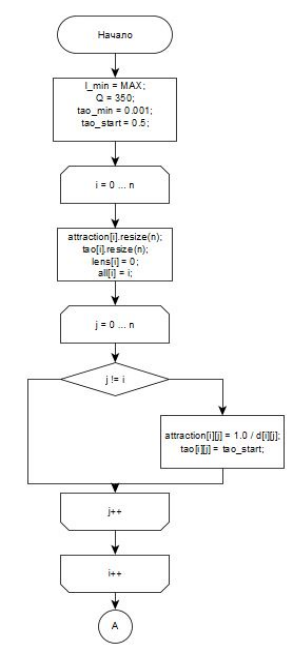
\includegraphics[scale=1]{img/formic.png}
			\caption{Схема муравьиного алгоритма часть 1.}
			\label{fig:formic1}
		\end{center}
	\end{figure}
	
	\begin{figure}[H]
		\begin{center}
			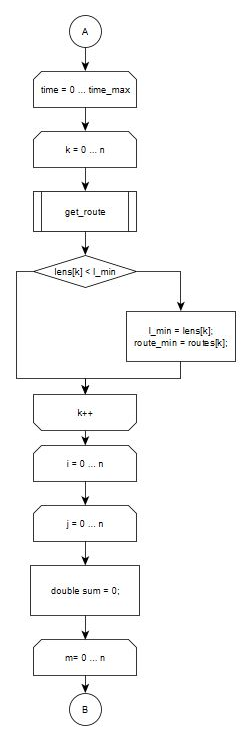
\includegraphics[scale=1]{img/formic2.png}
			\caption{Схема муравьиного алгоритма часть 2.}
			\label{fig:formic2}
		\end{center}
	\end{figure}
	
	\begin{figure}[H]
		\begin{center}
			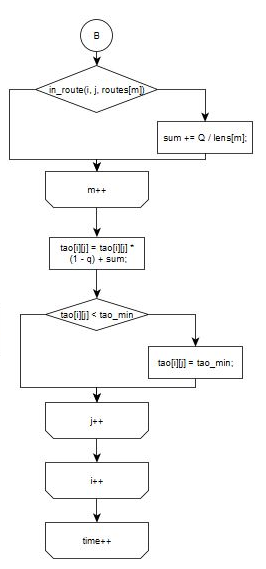
\includegraphics[scale=1]{img/formic3.png}
			\caption{Схема муравьиного алгоритма часть 3.}
			\label{fig:formic3}
		\end{center}
	\end{figure}
	
	На рисунках \ref{fig:en1}, \ref{fig:en2} представлена схема алгоритма полного перебора.
	\begin{figure}[H]
		\begin{center}
			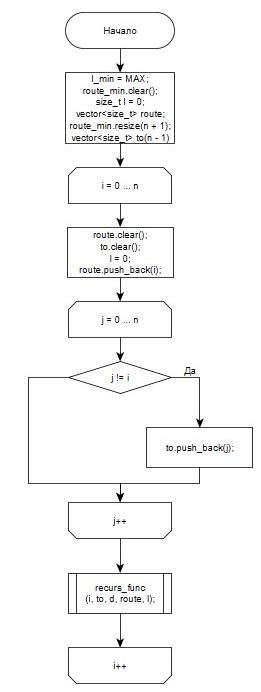
\includegraphics[scale=1]{img/enumeration1.png}
			\caption{Схема метода полного перебора часть 1.}
			\label{fig:en1}
		\end{center}
	\end{figure}
	
	\begin{figure}[H]
		\begin{center}
			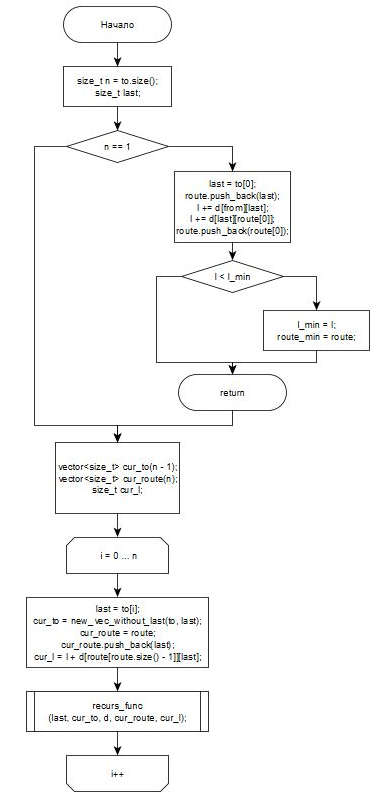
\includegraphics[scale=1]{img/enumeration2.png}
			\caption{Схема метода полного перебора часть 2.}
			\label{fig:en2}
		\end{center}
	\end{figure}
	
	\section*{Вывод}
	В данном разделе представлено описание архитектуры ПО и схемы муравьинного алгоритма и алгоритма перебором.
	
	\chapter{Технологическая часть}
	Данный раздел содержит обоснование выбора языка и среды разработки, реализацию алгоритмов.
	
	\section{Средства реализации}
	Для реализации программы был выбран язык программирования C++. Такой выбор обусловлен следующими причинами:
	\begin{itemize}
		\item имеет высокую производительность;
		\item наличие библиотек для удобной работы с векторами и замеров процессорного времени.
	\end{itemize}
	
	Для замера времени выполнения использовалась функция $clock()$ из библиотеки ctime. Эта функция возвращает количество временных тактов, прошедших с начала запуска программы ~\cite{cpp}. 
	
	\section{Реализация алгоритмов}
	В листингах \ref{lst:conv1} - \ref{lst:conv2} представлены реализации рассматриваемых алгоритмов.
	%\newpage
	\captionsetup{singlelinecheck=false, justification=raggedright}
	\begin{lstlisting}[label={lst:conv1},caption=Реализация алгоритма полного перебора (часть 1)]
		void recurs_func(size_t from, vector<size_t> to, vector<vector<size_t>> d, vector<size_t> route, size_t l) {
			
			size_t n = to.size();
			size_t last;
			if (n == 1) {
				last = to[0];
				route.push_back(last);
				l += d[from][last];
				l += d[last][route[0]];
				route.push_back(route[0]);
				if (l < l_min) {
					l_min = l;
					route_min = route;
				}
				return;
			}
		\end{lstlisting}
		\newpage
		\begin{lstlisting}[caption=Реализация алгоритма полного перебора (часть 2)]
			vector<size_t> cur_to(n - 1);
			vector<size_t> cur_route(n);
			size_t cur_l;
			for (size_t i = 0; i < n; i++) {
				last = to[i];
				cur_to = new_vec_without_last(to, last);
				cur_route = route;
				cur_route.push_back(last);
				cur_l = l + d[route[route.size() - 1]][last];
				recurs_func(last, cur_to, d, cur_route, cur_l);
			}
			
		}
		
		void perebor(size_t n, vector<vector<size_t>> d) {
			l_min = MAX;
			route_min.clear();
			size_t l = 0;
			vector<size_t> route;
			route_min.resize(n + 1);
			vector<size_t> to(n - 1);
			
			for (size_t i = 0; i < n; i++) {
				route.clear();
				to.clear();
				l = 0;
				
				route.push_back(i);
				for (size_t j = 0; j < n; j++)
				if (j != i)
				to.push_back(j);
				recurs_func(i, to, d, route, l);
			}
			
			cout << endl << "ROUTE: ";
			print_arr(route_min);
			cout << "LENGTH: " << l_min << endl << endl;
		}
	\end{lstlisting}
	\newpage
	\begin{lstlisting}[label={lst:conv1},caption=Реализация муравьиного алгоритма(часть 1)]
		vector<double> get_probability(size_t from, vector<size_t> to, vector<vector<double>> tao, vector<vector<double>> attraction,
		size_t alpha, size_t beta) {
			
			double znam = 0, chisl = 0;
			size_t n = to.size();
			vector<double> result(n);
			for (size_t i = 0; i < n; i++) {
				znam += pow(tao[from][to[i]], alpha) * pow(attraction[from][to[i]], beta);
			}
			for (size_t j = 0; j < n; j++) {
				chisl = pow(tao[from][to[j]], alpha) * pow(attraction[from][to[j]], beta);
				result[j] = chisl / znam;
			}
			return result;
		}
		
		void get_route(vector<size_t> all, size_t start, vector<size_t> &route, size_t &len, vector<vector<size_t>> d,
		vector<vector<double>> tao, vector<vector<double>> attraction,
		size_t alpha, size_t beta) {
			
			route.resize(0);
			route.push_back(start);
			vector<size_t> to = new_vec_without_last(all, start);
			size_t n_1 = tao.size() - 2;
			size_t from;
			double coin, sum;
			bool flag;
			
			for (size_t i = 0; i < n_1; i++) {
				sum = 0;
				flag = true;
				from = route[i];
				vector<double> p = get_probability(from, to, tao, attraction, alpha, beta);
				coin = double(rand() % 10000) / 10000;
			\end{lstlisting}
			\newpage\begin{lstlisting}[label={lst:conv1},caption=Реализация муравьиного алгоритма(часть 2)]
				for (size_t j = 0; j < p.size() && flag; j++) {
					sum += p[j];
					if (coin < sum) {
						route.push_back(to[j]);
						len += d[from][to[j]];
						to = new_vec_without_last(to, to[j]);
						flag = false;
					}
				}
			}
			len += d[route[route.size() - 1]][to[0]];
			route.push_back(to[0]);
			len += d[route[route.size() - 1]][route[0]];
			route.push_back(route[0]);
		}
		
		void ant(size_t n, vector<vector<size_t>> d, size_t alpha, size_t beta, double q, size_t time_max) {
			
			l_min = MAX;
			route_min.clear();
			
			double tao_min, tao_start, Q;
			vector<size_t> all(n);
			Q = 350;
			tao_min = 0.001;
			tao_start = 0.5;
			
			vector<vector<size_t>> routes(n);
			vector<size_t> lens(n);
			
			vector<vector<double>> attraction(n);
			vector<vector<double>> tao(n);
			
			for (size_t i = 0; i < n; i++) {
				attraction[i].resize(n);
				tao[i].resize(n);
				lens[i] = 0;
				all[i] = i;
			\end{lstlisting}
			\newpage
			\begin{lstlisting}[label={lst:conv2},caption=Реализация муравьиного алгоритма(часть 3)]
				for (size_t j = 0; j < n; j++) {
					if (i != j) {
						attraction[i][j] = 1.0 / d[i][j];
						tao[i][j] = tao_start;
					}
				}
			}
			
			for (size_t time = 0; time < time_max; time++) {
				for (size_t k = 0; k < n; k++) {
					get_route(all, k, routes[k], lens[k], d, tao, attraction, alpha, beta);
					if (lens[k] < l_min) {
						l_min = lens[k];
						route_min = routes[k];
					}
				}
				for (size_t i = 0; i < n; i++)
				for (size_t j = 0; j < n; j++) {
					double sum = 0;
					for (size_t m = 0; m < n; m++) {
						if (in_route(i, j, routes[m]))
						sum += Q / lens[m];
					}
					
					tao[i][j] = tao[i][j] * (1 - q) + sum;
					if (tao[i][j] < tao_min)
					tao[i][j] = tao_min;
				}
			}
		}
	\end{lstlisting}
	
	\section{Функциональные тесты}
	
	В первом столбце таблицы \ref{tab3} представлена матрица расстояний, во втором --- длина кратчайшего пути и сам кратчайший путь, в третьем --- найденная длина кратчайшего пути алгоритмом полного перебора и муравьиного алгоритма. На больших матрицах (от $5\times5$) результат работы муравьиного алгоритма может быть неточен. 
	
	
	\begin{table}[H]
		\caption{Функциональные тесты}
		\label{tab3}
		\begin{center}
			\begin{tabular}{ | c | c | c |}
				\hline
				\textbf{Матрица} & \textbf{Ожидаемая l и путь} & \textbf{Фактическая l и путь} \\ \hline
				$\begin{bmatrix} 
					0&3&4&4\\
					3&0&2&2\\
					4&2&0&3\\
					4&2&3&0
				\end{bmatrix}$ & 
				12, [1, 2, 3, 4, 1]
				& 
				12, [1, 4, 2, 3, 1] \\
				
				\hline
				$\begin{bmatrix} 
					0&167&116&56\\ 
					167&0&152&36 \\
					116&152&0&55\\
					56&36&55&0
				\end{bmatrix}$ & 
				288, [1, 3, 2, 4, 1]
				& 
				288, [2, 4, 1, 3, 2] \\
				
				\hline
				$\begin{bmatrix} 
					0&6312&9351\\
					6312&0&9127\\
					9351&9127&0
				\end{bmatrix}$ & 
				24790, [1, 2, 3, 1]
				& 
				24790, [1, 2, 3, 1] \\
				
				\hline
				
			\end{tabular}
			
		\end{center}
	\end{table} 
	Фактические результаты тестов совпали с ожидаемыми результатами.
	
	\section*{Вывод}
	В этом разделе обоснован выбор языка програмирования, описаны технические характеристики,приведены листинги кода реализованных алгоритмов и проведены функциональные тесты.
	\newpage
	
	\chapter{Экспериментальная часть}
	В данном разделе сравниваются реализованные алгоритмы, дается сравнительная оценка затрат на время.
	
	\section{Пример работы программы}
	Пример работы программы представлен на рисунке \ref{fig:ex}. На вход подаётся файл с матрицей расстояний. Результат работы муравьиного алгоритма записывается в файл, один из вариантов выводится в консоль. Пример файла в приложении 1.
	\captionsetup{singlelinecheck=true}
	\begin{figure}[H]
		\centering
		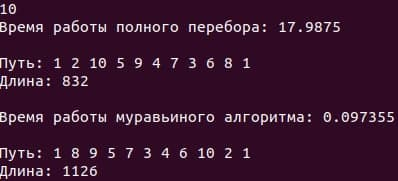
\includegraphics[width=1\linewidth]{img/ex}
		\caption{Пример работы программы}
		\label{fig:ex}
	\end{figure}
	
	\section{Технические характеристики}
	Технические характеристики устройства, на котором выполнялось исследование:
	\begin{itemize}
		\item операционная система: Windows~\cite{windows} 10 64-bit;;
		\item оперативная память: 16 Гб;
		\item процессор: Intel(R) Core(TM) i5-7600 CPU @ 3.50GHz \cite{i5}.
	\end{itemize}
	
	\section{Время выполнения алгоритмов}
	Был проведен сравнительный анализ реализаций муравьиного алгоритма и полного перебора. Замеры времени проводились для графов с количеством вершин от 2 до 10 с шагом 1. Значения коэффициентов составили $\alpha$ = 0, $t_{max}$ = 50, $\rho$ = 0.1.\\
	Результаты представлены в таблице \ref{tab2}:\\
	
	\begin{table}[H]
		\caption{Результаты замеров времени для алгоритма полного перебора и муравьиного алгоритма}
		\begin{center}
			\label{tab2}
			\begin{tabular}{|c|c|c|}
				\hline
				Количество вершин &Полный перебор& Муравьиный алгоритм \\\hline
				2&0.00001&0.00041\\
				3&0.00004&0.00096\\
				4&0.0002&0.002\\
				5&0.00053&0.0034\\
				6&0.0026&0.0062\\
				7&0.0175&0.0095\\
				8&0.13&0.013\\
				9&1.41&0.02\\
				10&14.88&0.027\\
				\hline
			\end{tabular}
		\end{center}
	\end{table} 
	
	\begin{center}
		\begin{tikzpicture}
			\begin{axis}[
				xlabel={Разница времени выполнения алгоритмов},
				ylabel={Время в секундах},
				xmin = 0, xmax = 10,
				ymin = 0, ymax = 20,
				legend pos=north west,
				ymajorgrids=true,
				grid style=dashed,
				]
				\legend{ 
					Алгоритм полного перебора,
					Муравьиный алгоритм
				}
				\addplot[
				color=yellow,
				mark=square,
				]
				coordinates {
					(2, 0.00001)
					(3, 0.00004)
					(4, 0.0002)
					(5, 0.00053)
					(6, 0.0026)
					(7, 0.0175)
					(8, 0.13)
					(9, 1.41)
					(10, 14.88)
				};
				\addplot[
				color=red,
				mark=square,
				]
				coordinates {
					(2, 0.00041)
					(3, 0.00096)
					(4, 0.002)
					(5, 0.0034)
					(6, 0.0062)
					(7, 0.0095)
					(8, 0.013)
					(9, 0.02)
					(10, 0.027)
				};
			\end{axis}
		\end{tikzpicture}
	\end{center}
	
	\section{Параметризация муравьиного алгоритма на основании проведенного эксперимента}	
	
	Работа муравьиного алгоритма зависит от параметров $\alpha$, $\beta$, $\rho$ и $t_{max}$. Найдем такие из них, при которых метод дает наиболее точный результат для трех классов данных (матрицы 10$\times$10).
	
	Параметр $\alpha$ будем варьировать от 0 до 1 с шагом 0.25, $\rho$  - от 0.1 до 0.9 с шагом 0.1, $t_{max}$ - от 50 до 400 с шагом 50. Результат тестирования - таблица со значениями $\alpha, \beta, \rho, t_{max}, \Delta L_{1}, \Delta L_{2}, \Delta L_{3}$, где $\delta L_{i}$ - разность эталонного решения задачи, полученного методом полного перебора, и полученного в процессе выполнения с заданными параметрами решения на $i$-м классе данных\\
	
	\subsection*{Класс данных 1}
	Первый класс данных \ref{mat:d1} - матрица смежности $10\times10$, элементы которой находятся в диапазоне $[1;4]$
	
	\begin{equation}
		\label{mat:d1}
		M = 
		\begin{pmatrix} 
			0 & 1 & 3 & 2 & 1 & 3 & 2 & 4 & 1 & 2 \\
			1 & 0 & 1 & 3 & 2 & 1 & 2 & 1 & 1 & 2 \\
			3 & 1 & 0 & 1 & 2 & 1 & 1 & 2 & 3 & 1 \\
			2 & 3 & 1 & 0 & 1 & 2 & 1 & 2 & 1 & 1 \\
			1 & 2 & 2 & 1 & 0 & 2 & 2 & 1 & 2 & 2 \\
			3 & 1 & 1 & 2 & 2 & 0 & 1 & 1 & 2 & 1 \\
			2 & 2 & 1 & 1 & 2 & 1 & 0 & 3 & 2 & 3 \\
			4 & 1 & 2 & 2 & 1 & 2 & 3 & 0 & 1 & 4 \\
			1 & 1 & 3 & 1 & 2 & 2 & 2 & 1 & 0 & 1 \\
			2 & 2 & 1 & 1 & 2 & 1 & 3 & 4 & 1 & 0
		\end{pmatrix}
	\end{equation}
	
	\subsection*{Класс данных 2}
	Второй класс данных \ref{mat:d2} - матрица смежности $10\times10$, элементы которой находятся в диапазоне $[11;1245]$
	
	\begin{equation}
		\label{mat:d2}
		M = 
		\begin{pmatrix} 
			0& 123& 32& 221& 125& 321& 542& 11& 122& 211\\ 
			123& 0& 123& 221& 122& 322& 221& 333& 321& 11\\ 
			32& 123& 0& 15& 443& 111& 45& 890& 326& 91\\ 
			221& 221& 15& 0& 543& 121& 55& 555& 98& 398\\ 
			125& 122& 443& 543& 0& 543& 232& 919& 111& 123\\
			321& 322& 111& 121& 543& 0& 554& 144& 1244& 243\\ 
			542& 221& 45& 55& 232& 554& 0& 321& 877& 577\\ 
			11& 333& 890& 555& 919& 144& 321& 0& 214& 612\\ 
			122& 321& 326& 98& 111& 1244& 877& 214& 0& 432\\
			211& 11& 91& 398& 123& 243& 577& 612& 432& 0
		\end{pmatrix}
	\end{equation}
	
	\subsection*{Класс данных 3}
	Третий класс данных \ref{mat:d3} - матрица смежности $10\times10$, элементы которой находятся в диапазоне $[5000;10000]$
	
	\begin{equation}
		\label{mat:d3}
		M = 
		\begin{pmatrix} 
			0& 6223& 9593& 6157& 6109& 8744& 7815& 9788& 7473& 9521\\
			6223& 0& 9200& 6017& 9634& 9532& 7447& 7114& 5762& 7713\\
			9593& 9200& 0& 6973& 6016& 7742& 7759& 8765& 6669& 9887\\
			6157& 6017& 6973& 0& 9973& 5432& 5906& 9754& 9715& 7519\\
			6109& 9634& 6016& 9973& 0& 6886& 7409& 6351& 7167& 9262\\
			8744& 9532& 7742& 5432& 6886& 0& 7663& 8084& 6900& 5081\\
			7815& 7447& 7759& 5906& 7409& 7663& 0& 8304& 9912& 5207\\
			9788& 7114& 8765& 9754& 6351& 8084& 8304& 0& 5984& 9808\\
			7473& 5762& 6669& 9715& 7167& 6900& 9912& 5984& 0& 7524\\
			9521& 7713& 9887& 7519& 9262& 5081& 5207& 9808& 7524& 0
		\end{pmatrix}
	\end{equation}
	
	Для каждого из классов данных были получены оптимальные сочетания параметров, представленные в таблицах \ref{tab:m1}-\ref{tab:m3}.
	
	\begin{table}[H]
		\caption{Оптимальные параметры для класса данных 1}
		\label{tab:m1}
		\begin{center}
			\begin{tabular}{|c|c|c|c|c|}
				\hline
				$t_{max}$ & $\alpha$ & $\beta$ & $\rho$ & $\Delta L_{1}$\\
				\hline
				50&0&1&0.4&0\\
				150&0&1&0.4&0\\
				150&0&1&0.6&0\\
				200&0&1&0.9&0\\
				\hline
			\end{tabular}
		\end{center}
	\end{table} 
	\begin{table}[H]
		\caption{Оптимальные параметры для класса данных 2}
		\label{tab:m2}
		\begin{center}
			\begin{tabular}{|c|c|c|c|c|}
				\hline
				$t_{max}$ & $\alpha$ & $\beta$ & $\rho$ & $\Delta L_{2}$\\
				\hline
				50&0&1&0.6&0\\
				\hline
			\end{tabular}
		\end{center}
	\end{table} 
	\begin{table}[H]
		\caption{Оптимальные параметры для класса данных 3}
		\label{tab:m3}
		\begin{center}
			\begin{tabular}{|c|c|c|c|c|}
				\hline
				$t_{max}$ & $\alpha$ & $\beta$ & $\rho$ & $\Delta L_{3}$ \\
				\hline
				250&0&1&0.5&0\\
				\hline
			\end{tabular}
		\end{center}
	\end{table} 
	
	Из полученных таблиц общими значениями параметров для оптимальных наборов являются $\alpha = 0$, $\beta = 1$. Для первого и второго классов данных общим является набор $\alpha = 0$, $\beta = 1$, $\rho = 0.6$.
	
	\section*{Вывод}
	По результатам исследования времени выполнения алгоритмов было выявлено, что при количестве вершин графа от 2 до 6, эффективнее использовать алгоритм полного перебора (преимущество составляет от 2.4 до 41 раз с уменьшением выигрыша при увеличении количества вершин графа).
	При большем количестве вершин выгоднее использовать муравьиный алгоритм, преимущество которого составляет от 1.8 до 551 раза с увеличением разрыва при увеличении количества вершин.
	
	Для заданных классов данных найдены параметры, которые обеспечивают наиболее оптимальное решение, для всех трех классов общими являются значения $\alpha = 0$, $\beta = 1$, для первого и второго - $\alpha = 0$, $\beta = 1$, $\rho = 0.6$.
	\newpage
	
	\addcontentsline{toc}{chapter}{Заключение}
	\chapter*{Заключение}
	В процессе выполнения лабораторной работы был проведен анализ метода полного перебора и эвристического метода на базе муравьиного алгоритма.
	
	Приведены схемы и реализованы программно алгоритм полного перебора и муравьиный алгоритм для решения задачи коммивояжера, проведено тестирование и параметризация муравьиного алгоритма для выбранного класса задач.
	
	По результатам исследования времени работы алгоритмов выявлено, что на графах, количество вершин которого находится в диапазоне от 2 до 6, эффективнее использовать метод полного перебора (выигрыш составляет от 2.4 до 41 раза с уменьшением при увеличении количества вершин), на больших графах - муравьиный алгоритм, преимущество которого составляет от 1.8 до 551 раза с увеличением разрыва при увеличении количества вершин.
	
	Общим для трех классов данных, приведенных в работе, стало сочетание параметров $\alpha$ и $\beta$ со значениями 0 и 1 соответственно, для первого и второго - $\alpha = 0$, $\beta = 1$, $\rho = 0.6$.
	\newpage
	\addcontentsline{toc}{chapter}{Список литературы}
	
	\bibliographystyle{utf8gost705u}
	\bibliography{report_6}
	\nocite{*}
	\chapter*{Приложение}
	В таблице \ref{tbl:only1}-\ref{tbl:only12} выводятся варьируемые параметры. Эталонная длина пути для первого класса данных - 10, для второго - 832, для третьего - 59972.
	\addcontentsline{toc}{chapter}{Приложение}
	\begin{table}[H]
		\begin{center}
			\captionsetup{justification=raggedright, singlelinecheck=false}
			\caption[]{\label{tbl:only1} Время выполнения полного перебора и муравьиного алгоритма}
			\begin{tabular}{|c|c|c|c|c|c|c|}
				\hline
				$t_{max}$ & $\alpha$ & $\beta$ & $\rho$ & $\Delta L_{1}$ & $\Delta L_{2}$ & $\Delta L_{3}$ \\
				\hline
				50 & 0 & 1 & 0.1 & 4 & 321 & 8756 \\
				50 & 0 & 1 & 0.2 & 1 & 664 & 5297 \\
				50 & 0 & 1 & 0.3 & 3 & 361 & 7229 \\
				50 & 0 & 1 & 0.4 & 0 & 120 & 7739 \\
				50 & 0 & 1 & 0.5 & 2 & 671 & 2621 \\
				50 & 0 & 1 & 0.6 & 2 & 0 & 9526 \\
				50 & 0 & 1 & 0.7 & 1 & 92 & 7138 \\
				50 & 0 & 1 & 0.8 & 3 & 447 & 9391 \\
				50 & 0 & 1 & 0.9 & 3 & 203 & 10643 \\
				50 & 0.25 & 0.75 & 0.1 & 7 & 1577 & 11970 \\
				50 & 0.25 & 0.75 & 0.2 & 3 & 1075 & 9243 \\
				50 & 0.25 & 0.75 & 0.3 & 6 & 903 & 11356 \\
				50 & 0.25 & 0.75 & 0.4 & 4 & 1192 & 11864 \\
				50 & 0.25 & 0.75 & 0.5 & 6 & 1122 & 9709 \\
				50 & 0.25 & 0.75 & 0.6 & 4 & 958 & 7728 \\
				50 & 0.25 & 0.75 & 0.7 & 3 & 912 & 11084 \\
				50 & 0.25 & 0.75 & 0.8 & 6 & 865 & 4807 \\
				50 & 0.25 & 0.75 & 0.9 & 1 & 413 & 7714 \\
				50 & 0.5 & 0.5 & 0.1 & 4 & 1507 & 9125 \\
				50 & 0.5 & 0.5 & 0.2 & 1 & 1008 & 7965 \\
				50 & 0.5 & 0.5 & 0.3 & 6 & 1394 & 8290 \\
				50 & 0.5 & 0.5 & 0.4 & 5 & 1291 & 9739 \\
				50 & 0.5 & 0.5 & 0.5 & 3 & 1323 & 11989 \\
				50 & 0.5 & 0.5 & 0.6 & 5 & 915 & 10797 \\
				50 & 0.5 & 0.5 & 0.7 & 4 & 1585 & 10430 \\
				50 & 0.5 & 0.5 & 0.8 & 2 & 1336 & 9237 \\
				50 & 0.5 & 0.5 & 0.9 & 4 & 1562 & 10257 \\
				50 & 0.75 & 0.25 & 0.1 & 3 & 1774 & 10032 \\
				50 & 0.75 & 0.25 & 0.2 & 1 & 906 & 12146 \\
				\hline
			\end{tabular}
		\end{center}
	\end{table}
	\newpage 
	
	\begin{table}[H]
		\begin{center}
			\caption[]{\label{tbl:only2} Время выполнения полного перебора и муравьиного алгоритма}
			\begin{tabular}{|c|c|c|c|c|c|c|}
				\hline
				$t_{max}$ & $\alpha$ & $\beta$ & $\rho$ & $\Delta L_{1}$ & $\Delta L_{2}$ & $\Delta L_{3}$\\
				\hline
				50 & 0.75 & 0.25 & 0.3 & 4 & 629 & 8357 \\
				50 & 0.75 & 0.25 & 0.4 & 4 & 1661 & 11174 \\
				50 & 0.75 & 0.25 & 0.5 & 4 & 1553 & 7463 \\
				50 & 0.75 & 0.25 & 0.6 & 5 & 1170 & 6883 \\
				50 & 0.75 & 0.25 & 0.7 & 3 & 991 & 13063 \\
				50 & 0.75 & 0.25 & 0.8 & 3 & 1223 & 10065 \\
				50 & 0.75 & 0.25 & 0.9 & 5 & 1334 & 14601 \\
				50 & 1 & 0 & 0.1 & 3 & 1124 & 11070 \\
				50 & 1 & 0 & 0.2 & 3 & 1382 & 8615 \\
				50 & 1 & 0 & 0.3 & 4 & 700 & 10180 \\
				50 & 1 & 0 & 0.4 & 5 & 722 & 7314 \\
				50 & 1 & 0 & 0.5 & 5 & 2130 & 10054 \\
				50 & 1 & 0 & 0.6 & 5 & 1261 & 5304 \\
				50 & 1 & 0 & 0.7 & 5 & 1604 & 7816 \\
				50 & 1 & 0 & 0.8 & 5 & 1430 & 12009 \\
				50 & 1 & 0 & 0.9 & 7 & 1444 & 12247 \\
				100 & 0 & 1 & 0.1 & 2 & 419 & 8045 \\
				100 & 0 & 1 & 0.2 & 2 & 212 & 8225 \\
				100 & 0 & 1 & 0.3 & 1 & 192 & 6189 \\
				100 & 0 & 1 & 0.4 & 1 & 270 & 7441 \\
				100 & 0 & 1 & 0.5 & 2 & 403 & 8734 \\
				100 & 0 & 1 & 0.6 & 3 & 240 & 9833 \\
				100 & 0 & 1 & 0.7 & 2 & 330 & 11453 \\
				100 & 0 & 1 & 0.8 & 3 & 155 & 8789 \\
				100 & 0 & 1 & 0.9 & 1 & 536 & 4731 \\
				100 & 0.25 & 0.75 & 0.1 & 4 & 1074 & 13862 \\
				100 & 0.25 & 0.75 & 0.2 & 4 & 950 & 10485 \\
				100 & 0.25 & 0.75 & 0.3 & 4 & 1421 & 10884 \\
				100 & 0.25 & 0.75 & 0.4 & 6 & 2041 & 10379 \\
				100 & 0.25 & 0.75 & 0.5 & 4 & 1016 & 12817 \\
				100 & 0.25 & 0.75 & 0.6 & 3 & 1311 & 11278 \\
				100 & 0.25 & 0.75 & 0.7 & 5 & 1234 & 11178 \\
				\hline
				
			\end{tabular}
		\end{center}
	\end{table}
	\begin{table}[H]
		\begin{center}
			\caption[]{\label{tbl:only3} Время выполнения полного перебора и муравьиного алгоритма}
			\begin{tabular}{|c|c|c|c|c|c|c|}
				\hline
				$t_{max}$ & $\alpha$ & $\beta$& $\rho$ & $\Delta L_{1}$ & $\Delta L_{2}$ & $\Delta L_{3}$\\
				\hline
				100 & 0.25 & 0.75 & 0.8 & 5 & 1424 & 8487 \\
				100 & 0.25 & 0.75 & 0.9 & 5 & 1384 & 9486 \\
				100 & 0.5 & 0.5 & 0.1 & 5 & 1397 & 10850 \\
				100 & 0.5 & 0.5 & 0.2 & 4 & 1376 & 11320 \\
				100 & 0.5 & 0.5 & 0.3 & 4 & 1009 & 9336 \\
				100 & 0.5 & 0.5 & 0.4 & 4 & 2038 & 15597 \\
				100 & 0.5 & 0.5 & 0.5 & 5 & 746 & 10422 \\
				100 & 0.5 & 0.5 & 0.6 & 5 & 1631 & 10750 \\
				100 & 0.5 & 0.5 & 0.7 & 3 & 1284 & 9855 \\
				100 & 0.5 & 0.5 & 0.8 & 4 & 745 & 10229 \\
				100 & 0.5 & 0.5 & 0.9 & 5 & 916 & 11513 \\
				100 & 0.75 & 0.25 & 0.1 & 6 & 2294 & 11655 \\
				100 & 0.75 & 0.25 & 0.2 & 6 & 1689 & 7774 \\
				100 & 0.75 & 0.25 & 0.3 & 4 & 1621 & 11845 \\
				100 & 0.75 & 0.25 & 0.4 & 4 & 1199 & 12541 \\
				100 & 0.75 & 0.25 & 0.5 & 3 & 1625 & 6353 \\
				100 & 0.75 & 0.25 & 0.6 & 3 & 1135 & 7644 \\
				100 & 0.75 & 0.25 & 0.7 & 4 & 1334 & 12616 \\
				100 & 0.75 & 0.25 & 0.8 & 5 & 1134 & 13450 \\
				100 & 0.75 & 0.25 & 0.9 & 3 & 832 & 10845 \\
				100 & 1 & 0 & 0.1 & 3 & 1235 & 13061 \\
				100 & 1 & 0 & 0.2 & 4 & 423 & 15478 \\
				100 & 1 & 0 & 0.3 & 7 & 890 & 10349 \\
				100 & 1 & 0 & 0.4 & 4 & 1406 & 8261 \\
				100 & 1 & 0 & 0.5 & 4 & 1425 & 9724 \\
				100 & 1 & 0 & 0.6 & 4 & 1558 & 12325 \\
				100 & 1 & 0 & 0.7 & 5 & 1343 & 10008 \\
				100 & 1 & 0 & 0.8 & 4 & 1008 & 11384 \\
				100 & 1 & 0 & 0.9 & 5 & 1268 & 8968 \\
				150 & 0 & 1 & 0.1 & 1 & 303 & 10707 \\
				150 & 0 & 1 & 0.2 & 3 & 92 & 8963 \\
				150 & 0 & 1 & 0.3 & 3 & 192 & 12567 \\
				\hline
				
			\end{tabular}
		\end{center}
	\end{table}
	\begin{table}[H]
		\begin{center}
			\caption[]{\label{tbl:only4} Время выполнения полного перебора и муравьиного алгоритма}
			\begin{tabular}{|c|c|c|c|c|c|c|}
				\hline
				$t_{max}$ & $\alpha$ & $\beta$ &$\rho$ & $\Delta L_{1}$ & $\Delta L_{2}$ & $\Delta L_{3}$\\
				\hline		150 & 0 & 1 & 0.4 & 0 & 481 & 9986 \\
				150 & 0 & 1 & 0.5 & 2 & 120 & 10886 \\
				150 & 0 & 1 & 0.6 & 0 & 430 & 10750 \\
				150 & 0 & 1 & 0.7 & 3 & 333 & 6854 \\
				150 & 0 & 1 & 0.8 & 4 & 544 & 9940 \\
				150 & 0 & 1 & 0.9 & 2 & 120 & 12593 \\
				150 & 0.25 & 0.75 & 0.1 & 3 & 913 & 12235 \\
				150 & 0.25 & 0.75 & 0.2 & 3 & 1238 & 12767 \\
				150 & 0.25 & 0.75 & 0.3 & 4 & 1625 & 13750 \\
				150 & 0.25 & 0.75 & 0.4 & 4 & 1991 & 9691 \\
				150 & 0.25 & 0.75 & 0.5 & 3 & 1449 & 5898 \\
				150 & 0.25 & 0.75 & 0.6 & 5 & 1522 & 6929 \\
				150 & 0.25 & 0.75 & 0.7 & 2 & 1630 & 13159 \\
				150 & 0.25 & 0.75 & 0.8 & 4 & 1541 & 11210 \\
				150 & 0.25 & 0.75 & 0.9 & 4 & 1170 & 11096 \\
				150 & 0.5 & 0.5 & 0.1 & 2 & 1099 & 5728 \\
				150 & 0.5 & 0.5 & 0.2 & 6 & 1977 & 13189 \\
				150 & 0.5 & 0.5 & 0.3 & 3 & 1183 & 10272 \\
				150 & 0.5 & 0.5 & 0.4 & 3 & 1203 & 10083 \\
				150 & 0.5 & 0.5 & 0.5 & 3 & 716 & 14089 \\
				150 & 0.5 & 0.5 & 0.6 & 4 & 294 & 8969 \\
				150 & 0.5 & 0.5 & 0.7 & 5 & 1754 & 9116 \\
				150 & 0.5 & 0.5 & 0.8 & 3 & 1977 & 9097 \\
				150 & 0.5 & 0.5 & 0.9 & 3 & 715 & 9854 \\
				150 & 0.75 & 0.25 & 0.1 & 6 & 1728 & 6526 \\
				150 & 0.75 & 0.25 & 0.2 & 4 & 1458 & 11115 \\
				150 & 0.75 & 0.25 & 0.3 & 4 & 1465 & 14121 \\
				150 & 0.75 & 0.25 & 0.4 & 3 & 675 & 5651 \\
				150 & 0.75 & 0.25 & 0.5 & 2 & 987 & 7760 \\
				150 & 0.75 & 0.25 & 0.6 & 3 & 1143 & 8571 \\
				150 & 0.75 & 0.25 & 0.7 & 6 & 970 & 11273 \\
				\hline	
			\end{tabular}
		\end{center}
	\end{table}
	\begin{table}[H]
		\begin{center}
			\caption[]{\label{tbl:only5} Время выполнения полного перебора и муравьиного алгоритма}
			\begin{tabular}{|c|c|c|c|c|c|c|}
				\hline
				$t_{max}$ & $\alpha$ & $\beta$ & $\rho$ & $\Delta L_{1}$ & $\Delta L_{2}$ & $\Delta L_{3}$\\
				\hline
				150 & 0.75 & 0.25 & 0.8 & 4 & 1373 & 13305 \\
				150 & 0.75 & 0.25 & 0.9 & 6 & 1218 & 11096 \\
				150 & 1 & 0 & 0.1 & 4 & 1274 & 5786 \\
				150 & 1 & 0 & 0.2 & 3 & 1434 & 12328 \\
				150 & 1 & 0 & 0.3 & 2 & 1166 & 9063 \\
				150 & 1 & 0 & 0.4 & 4 & 1748 & 10983 \\
				150 & 1 & 0 & 0.5 & 3 & 1596 & 12162 \\
				150 & 1 & 0 & 0.6 & 4 & 1267 & 11352 \\
				150 & 1 & 0 & 0.7 & 4 & 902 & 8041 \\
				150 & 1 & 0 & 0.8 & 5 & 895 & 13259 \\
				150 & 1 & 0 & 0.9 & 2 & 942 & 9467 \\
				200 & 0 & 1 & 0.1 & 1 & 265 & 8665 \\
				200 & 0 & 1 & 0.2 & 5 & 404 & 9355 \\
				200 & 0 & 1 & 0.3 & 2 & 367 & 11411 \\
				200 & 0 & 1 & 0.4 & 2 & 413 & 7964 \\
				200 & 0 & 1 & 0.5 & 3 & 1 & 10293 \\
				200 & 0 & 1 & 0.6 & 3 & 488 & 8838 \\
				200 & 0 & 1 & 0.7 & 2 & 40 & 10818 \\
				200 & 0 & 1 & 0.8 & 2 & 480 & 8376 \\
				200 & 0 & 1 & 0.9 & 0 & 480 & 9213 \\
				200 & 0.25 & 0.75 & 0.1 & 4 & 1521 & 10179 \\
				200 & 0.25 & 0.75 & 0.2 & 4 & 1025 & 12307 \\
				200 & 0.25 & 0.75 & 0.3 & 3 & 998 & 10767 \\
				200 & 0.25 & 0.75 & 0.4 & 4 & 1289 & 11705 \\
				200 & 0.25 & 0.75 & 0.5 & 5 & 799 & 5578 \\
				200 & 0.25 & 0.75 & 0.6 & 3 & 1284 & 8426 \\
				200 & 0.25 & 0.75 & 0.7 & 3 & 1045 & 10055 \\
				200 & 0.25 & 0.75 & 0.8 & 5 & 1865 & 7466 \\
				200 & 0.25 & 0.75 & 0.9 & 4 & 740 & 9829 \\
				200 & 0.5 & 0.5 & 0.1 & 5 & 1038 & 10106 \\
				200 & 0.5 & 0.5 & 0.2 & 6 & 1070 & 9479 \\
				200 & 0.5 & 0.5 & 0.3 & 4 & 1362 & 6692 \\
				\hline
			\end{tabular}
		\end{center}
	\end{table}
	\begin{table}[H]
		\begin{center}
			\caption[]{\label{tbl:only6} Время выполнения полного перебора и муравьиного алгоритма}
			\begin{tabular}{|c|c|c|c|c|c|c|}
				\hline
				$t_{max}$ & $\alpha$ & $\beta$&$\rho$ &$\Delta L_{1}$ & $\Delta L_{2}$ & $\Delta L_{3}$\\
				\hline
				200 & 0.5 & 0.5 & 0.4 & 5 & 876 & 11640 \\
				200 & 0.5 & 0.5 & 0.5 & 3 & 919 & 11724 \\
				200 & 0.5 & 0.5 & 0.6 & 5 & 1366 & 8644 \\
				200 & 0.5 & 0.5 & 0.7 & 2 & 1346 & 11620 \\
				200 & 0.5 & 0.5 & 0.8 & 5 & 760 & 12334 \\
				200 & 0.5 & 0.5 & 0.9 & 4 & 1021 & 11323 \\
				200 & 0.75 & 0.25 & 0.1 & 2 & 2072 & 13053 \\
				200 & 0.75 & 0.25 & 0.2 & 6 & 1564 & 11677 \\
				200 & 0.75 & 0.25 & 0.3 & 4 & 1500 & 14739 \\
				200 & 0.75 & 0.25 & 0.4 & 4 & 918 & 12991 \\
				200 & 0.75 & 0.25 & 0.5 & 2 & 1160 & 10307 \\
				200 & 0.75 & 0.25 & 0.6 & 4 & 1155 & 4186 \\
				200 & 0.75 & 0.25 & 0.7 & 5 & 1259 & 6158 \\
				200 & 0.75 & 0.25 & 0.8 & 5 & 1072 & 5530 \\
				200 & 0.75 & 0.25 & 0.9 & 3 & 1546 & 11670 \\
				200 & 1 & 0 & 0.1 & 6 & 696 & 13300 \\
				200 & 1 & 0 & 0.2 & 6 & 1440 & 10068 \\
				200 & 1 & 0 & 0.3 & 4 & 924 & 9860 \\
				200 & 1 & 0 & 0.4 & 2 & 1030 & 10056 \\
				200 & 1 & 0 & 0.5 & 4 & 1215 & 12340 \\
				200 & 1 & 0 & 0.6 & 3 & 1448 & 8777 \\
				200 & 1 & 0 & 0.7 & 3 & 836 & 9864 \\
				200 & 1 & 0 & 0.8 & 5 & 1357 & 8828 \\
				200 & 1 & 0 & 0.9 & 4 & 1257 & 9179 \\
				250 & 0 & 1 & 0.1 & 1 & 698 & 10571 \\
				250 & 0 & 1 & 0.2 & 2 & 515 & 9265 \\
				250 & 0 & 1 & 0.3 & 2 & 92 & 6415 \\
				250 & 0 & 1 & 0.4 & 2 & 298 & 5168 \\
				250 & 0 & 1 & 0.5 & 2 & 235 & 0 \\
				250 & 0 & 1 & 0.6 & 2 & 683 & 9342 \\
				250 & 0 & 1 & 0.7 & 2 & 40 & 9962 \\
				250 & 0 & 1 & 0.8 & 1 & 211 & 8398 \\
				\hline	
			\end{tabular}
		\end{center}
	\end{table}
	\begin{table}[H]
		\begin{center}
			\caption[]{\label{tbl:only7} Время выполнения полного перебора и муравьиного алгоритма}
			\begin{tabular}{|c|c|c|c|c|c|c|}
				\hline
				$t_{max}$ & $\alpha$ & $\beta$ &$\rho$ & $\Delta L_{1}$ & $\Delta L_{2}$ & $\Delta L_{3}$\\
				\hline
				250 & 0 & 1 & 0.9 & 3 & 133 & 8469 \\
				250 & 0.25 & 0.75 & 0.1 & 5 & 1114 & 4043 \\
				250 & 0.25 & 0.75 & 0.2 & 5 & 1248 & 10064 \\
				250 & 0.25 & 0.75 & 0.3 & 3 & 1426 & 9732 \\
				250 & 0.25 & 0.75 & 0.4 & 5 & 933 & 10577 \\
				250 & 0.25 & 0.75 & 0.5 & 4 & 1185 & 8709 \\
				250 & 0.25 & 0.75 & 0.6 & 3 & 1638 & 9928 \\
				250 & 0.25 & 0.75 & 0.7 & 4 & 777 & 7512 \\
				250 & 0.25 & 0.75 & 0.8 & 2 & 1653 & 10007 \\
				250 & 0.25 & 0.75 & 0.9 & 2 & 1048 & 4108 \\
				250 & 0.5 & 0.5 & 0.1 & 4 & 901 & 10118 \\
				250 & 0.5 & 0.5 & 0.2 & 4 & 966 & 7825 \\
				250 & 0.5 & 0.5 & 0.3 & 5 & 1490 & 17096 \\
				250 & 0.5 & 0.5 & 0.4 & 4 & 1296 & 10505 \\
				250 & 0.5 & 0.5 & 0.5 & 3 & 790 & 6406 \\
				250 & 0.5 & 0.5 & 0.6 & 3 & 1200 & 10748 \\
				250 & 0.5 & 0.5 & 0.7 & 3 & 1287 & 11191 \\
				250 & 0.5 & 0.5 & 0.8 & 3 & 1341 & 9400 \\
				250 & 0.5 & 0.5 & 0.9 & 5 & 1746 & 10785 \\
				250 & 0.75 & 0.25 & 0.1 & 3 & 1340 & 11007 \\
				250 & 0.75 & 0.25 & 0.2 & 6 & 888 & 8637 \\
				250 & 0.75 & 0.25 & 0.3 & 6 & 848 & 8354 \\
				250 & 0.75 & 0.25 & 0.4 & 4 & 1583 & 8246 \\
				250 & 0.75 & 0.25 & 0.5 & 3 & 939 & 12496 \\
				250 & 0.75 & 0.25 & 0.6 & 4 & 1785 & 12991 \\
				250 & 0.75 & 0.25 & 0.7 & 3 & 1245 & 6608 \\
				250 & 0.75 & 0.25 & 0.8 & 2 & 1609 & 11078 \\
				250 & 0.75 & 0.25 & 0.9 & 5 & 976 & 9056 \\
				250 & 1 & 0 & 0.1 & 5 & 923 & 9767 \\
				250 & 1 & 0 & 0.2 & 5 & 1433 & 6779 \\
				250 & 1 & 0 & 0.3 & 5 & 1302 & 11255 \\
				250 & 1 & 0 & 0.4 & 5 & 998 & 11757 \\
				\hline
			\end{tabular}
		\end{center}
	\end{table}
	\begin{table}[H]
		\begin{center}
			\caption[]{\label{tbl:only8} Время выполнения полного перебора и муравьиного алгоритма}
			\begin{tabular}{|c|c|c|c|c|c|c|}
				\hline
				$t_{max}$ & $\alpha$ & $\beta$ & $\rho$ & $\Delta L_{1}$ & $\Delta L_{2}$ & $\Delta L_{3}$\\
				\hline
				250 & 1 & 0 & 0.5 & 5 & 2004 & 12309 \\
				250 & 1 & 0 & 0.6 & 4 & 1063 & 11136 \\
				250 & 1 & 0 & 0.7 & 6 & 1326 & 11957 \\
				250 & 1 & 0 & 0.8 & 2 & 758 & 9613 \\
				250 & 1 & 0 & 0.9 & 4 & 1122 & 10982 \\
				300 & 0 & 1 & 0.1 & 2 & 709 & 9937 \\
				300 & 0 & 1 & 0.2 & 3 & 34 & 7900 \\
				300 & 0 & 1 & 0.3 & 3 & 312 & 9466 \\
				300 & 0 & 1 & 0.4 & 2 & 290 & 8784 \\
				300 & 0 & 1 & 0.5 & 1 & 582 & 7761 \\
				300 & 0 & 1 & 0.6 & 3 & 297 & 8058 \\
				300 & 0 & 1 & 0.7 & 2 & 716 & 5535 \\
				300 & 0 & 1 & 0.8 & 1 & 482 & 6093 \\
				300 & 0 & 1 & 0.9 & 2 & 270 & 7984 \\
				300 & 0.25 & 0.75 & 0.1 & 5 & 1582 & 14106 \\
				300 & 0.25 & 0.75 & 0.2 & 4 & 390 & 2168 \\
				300 & 0.25 & 0.75 & 0.3 & 4 & 2084 & 6742 \\
				300 & 0.25 & 0.75 & 0.4 & 6 & 1040 & 13010 \\
				300 & 0.25 & 0.75 & 0.5 & 5 & 1567 & 11956 \\
				300 & 0.25 & 0.75 & 0.6 & 5 & 942 & 7115 \\
				300 & 0.25 & 0.75 & 0.7 & 6 & 1228 & 10068 \\
				300 & 0.25 & 0.75 & 0.8 & 5 & 1292 & 9606 \\
				300 & 0.25 & 0.75 & 0.9 & 5 & 1389 & 15772 \\
				300 & 0.5 & 0.5 & 0.1 & 2 & 1622 & 8551 \\
				300 & 0.5 & 0.5 & 0.2 & 6 & 1204 & 9348 \\
				300 & 0.5 & 0.5 & 0.3 & 3 & 1450 & 10386 \\
				300 & 0.5 & 0.5 & 0.4 & 3 & 1245 & 10203 \\
				300 & 0.5 & 0.5 & 0.5 & 3 & 1109 & 15642 \\
				300 & 0.5 & 0.5 & 0.6 & 3 & 1040 & 12369 \\
				300 & 0.5 & 0.5 & 0.7 & 4 & 1029 & 11515 \\
				300 & 0.5 & 0.5 & 0.8 & 4 & 1043 & 10118 \\
				300 & 0.5 & 0.5 & 0.9 & 5 & 1466 & 12997 \\
				\hline	
			\end{tabular}
		\end{center}
	\end{table}
	\begin{table}[H]
		\begin{center}
			\caption[]{\label{tbl:only9} Время выполнения полного перебора и муравьиного алгоритма}
			\begin{tabular}{|c|c|c|c|c|c|c|}
				\hline
				$t_{max}$ & $\alpha$ & $\beta$ &$\rho$ & $\Delta L_{1}$ & $\Delta L_{2}$ & $\Delta L_{3}$\\
				\hline
				300 & 0.75 & 0.25 & 0.1 & 5 & 1147 & 11937 \\
				300 & 0.75 & 0.25 & 0.2 & 3 & 1722 & 5690 \\
				300 & 0.75 & 0.25 & 0.3 & 4 & 1148 & 9056 \\
				300 & 0.75 & 0.25 & 0.4 & 2 & 981 & 8279 \\
				300 & 0.75 & 0.25 & 0.5 & 3 & 1048 & 9760 \\
				300 & 0.75 & 0.25 & 0.6 & 5 & 1495 & 9998 \\
				300 & 0.75 & 0.25 & 0.7 & 2 & 894 & 8841 \\
				300 & 0.75 & 0.25 & 0.8 & 3 & 815 & 13458 \\
				300 & 0.75 & 0.25 & 0.9 & 4 & 540 & 12323 \\
				300 & 1 & 0 & 0.1 & 2 & 1413 & 12086 \\
				300 & 1 & 0 & 0.2 & 2 & 1338 & 12370 \\
				300 & 1 & 0 & 0.3 & 5 & 695 & 14532 \\
				300 & 1 & 0 & 0.4 & 5 & 963 & 11282 \\
				300 & 1 & 0 & 0.5 & 5 & 1665 & 13379 \\
				300 & 1 & 0 & 0.6 & 5 & 1719 & 10666 \\
				300 & 1 & 0 & 0.7 & 2 & 1458 & 13796 \\
				300 & 1 & 0 & 0.8 & 5 & 1837 & 8800 \\
				300 & 1 & 0 & 0.9 & 3 & 1291 & 10831 \\
				350 & 0 & 1 & 0.1 & 3 & 444 & 7399 \\
				350 & 0 & 1 & 0.2 & 1 & 466 & 14815 \\
				350 & 0 & 1 & 0.3 & 3 & 235 & 11042 \\
				350 & 0 & 1 & 0.4 & 2 & 40 & 6752 \\
				350 & 0 & 1 & 0.5 & 1 & 92 & 6758 \\
				350 & 0 & 1 & 0.6 & 2 & 323 & 8775 \\
				350 & 0 & 1 & 0.7 & 1 & 240 & 11755 \\
				350 & 0 & 1 & 0.8 & 3 & 290 & 12144 \\
				350 & 0 & 1 & 0.9 & 4 & 248 & 7516 \\
				350 & 0.25 & 0.75 & 0.1 & 6 & 1321 & 14991 \\
				350 & 0.25 & 0.75 & 0.2 & 3 & 1060 & 10849 \\
				350 & 0.25 & 0.75 & 0.3 & 6 & 762 & 4781 \\
				350 & 0.25 & 0.75 & 0.4 & 5 & 1435 & 16012 \\
				350 & 0.25 & 0.75 & 0.5 & 5 & 1375 & 9661 \\
				
				\hline
			\end{tabular}
		\end{center}
	\end{table}
	\begin{table}[H]
		\begin{center}
			\caption[]{\label{tbl:only10} Время выполнения полного перебора и муравьиного алгоритма}
			\begin{tabular}{|c|c|c|c|c|c|c|}
				\hline
				$t_{max}$ & $\alpha$ & $\beta$ & $\rho$ & $\Delta L_{1}$ & $\Delta L_{2}$ & $\Delta L_{3}$\\
				\hline
				350 & 0.25 & 0.75 & 0.6 & 3 & 1218 & 13763 \\
				350 & 0.25 & 0.75 & 0.7 & 4 & 1647 & 9926 \\
				350 & 0.25 & 0.75 & 0.8 & 4 & 1254 & 6629 \\
				350 & 0.25 & 0.75 & 0.9 & 3 & 1420 & 9748 \\
				350 & 0.5 & 0.5 & 0.1 & 5 & 1087 & 7583 \\
				350 & 0.5 & 0.5 & 0.2 & 4 & 826 & 7038 \\
				350 & 0.5 & 0.5 & 0.3 & 3 & 1631 & 14789 \\
				350 & 0.5 & 0.5 & 0.4 & 5 & 1280 & 10748 \\
				350 & 0.5 & 0.5 & 0.5 & 4 & 1340 & 11922 \\
				350 & 0.5 & 0.5 & 0.6 & 4 & 1223 & 12277 \\
				350 & 0.5 & 0.5 & 0.7 & 4 & 741 & 9177 \\
				350 & 0.5 & 0.5 & 0.8 & 3 & 2575 & 11585 \\
				350 & 0.5 & 0.5 & 0.9 & 3 & 1077 & 10565 \\
				350 & 0.75 & 0.25 & 0.1 & 3 & 1110 & 6207 \\
				350 & 0.75 & 0.25 & 0.2 & 2 & 513 & 7815 \\
				350 & 0.75 & 0.25 & 0.3 & 5 & 1519 & 12731 \\
				350 & 0.75 & 0.25 & 0.4 & 4 & 1145 & 7312 \\
				350 & 0.75 & 0.25 & 0.5 & 5 & 1203 & 12719 \\
				350 & 0.75 & 0.25 & 0.6 & 5 & 1217 & 8659 \\
				350 & 0.75 & 0.25 & 0.7 & 6 & 1438 & 8160 \\
				350 & 0.75 & 0.25 & 0.8 & 4 & 1395 & 9522 \\
				350 & 0.75 & 0.25 & 0.9 & 2 & 1043 & 13698 \\
				350 & 1 & 0 & 0.1 & 5 & 811 & 8508 \\
				350 & 1 & 0 & 0.2 & 2 & 1507 & 14828 \\
				350 & 1 & 0 & 0.3 & 4 & 1470 & 14812 \\
				350 & 1 & 0 & 0.4 & 3 & 843 & 11712 \\
				350 & 1 & 0 & 0.5 & 5 & 1068 & 8061 \\
				350 & 1 & 0 & 0.6 & 4 & 648 & 10997 \\
				350 & 1 & 0 & 0.7 & 4 & 1679 & 7781 \\
				350 & 1 & 0 & 0.8 & 3 & 1623 & 12624 \\
				350 & 1 & 0 & 0.9 & 3 & 1541 & 11793 \\
				400 & 0 & 1 & 0.1 & 3 & 560 & 10642 \\
				\hline 	
			\end{tabular}
		\end{center}
	\end{table}
	\newpage
	\begin{table}[H]
		\begin{center}
			\caption[]{\label{tbl:only11} Время выполнения полного перебора и муравьиного алгоритма}
			\begin{tabular}{|c|c|c|c|c|c|c|}
				\hline
				$t_{max}$ & $\alpha$ & $\beta$ & $\rho$ & $\Delta L_{1}$ & $\Delta L_{2}$ & $\Delta L_{3}$\\
				\hline			
				400 & 0 & 1 & 0.2 & 2 & 533 & 5636 \\
				400 & 0 & 1 & 0.3 & 3 & 192 & 7931 \\
				400 & 0 & 1 & 0.4 & 3 & 461 & 11510 \\
				400 & 0 & 1 & 0.5 & 3 & 413 & 10950 \\
				400 & 0 & 1 & 0.6 & 4 & 578 & 3884 \\
				400 & 0 & 1 & 0.7 & 4 & 510 & 7366 \\
				400 & 0 & 1 & 0.8 & 1 & 507 & 1879 \\
				400 & 0 & 1 & 0.9 & 2 & 40 & 6831 \\
				400 & 0.25 & 0.75 & 0.1 & 2 & 1539 & 11958 \\
				400 & 0.25 & 0.75 & 0.2 & 4 & 1473 & 8810 \\
				400 & 0.25 & 0.75 & 0.3 & 3 & 1488 & 9461 \\
				400 & 0.25 & 0.75 & 0.4 & 6 & 828 & 10506 \\
				400 & 0.25 & 0.75 & 0.5 & 2 & 1765 & 13904 \\
				400 & 0.25 & 0.75 & 0.6 & 3 & 1811 & 13815 \\
				400 & 0.25 & 0.75 & 0.7 & 3 & 1118 & 11033 \\
				400 & 0.25 & 0.75 & 0.8 & 4 & 1502 & 7311 \\
				400 & 0.25 & 0.75 & 0.9 & 5 & 882 & 13035 \\
				400 & 0.5 & 0.5 & 0.1 & 6 & 1262 & 9966 \\
				400 & 0.5 & 0.5 & 0.2 & 1 & 1078 & 12274 \\
				400 & 0.5 & 0.5 & 0.3 & 4 & 1629 & 8690 \\
				400 & 0.5 & 0.5 & 0.4 & 3 & 1303 & 13380 \\
				400 & 0.5 & 0.5 & 0.5 & 4 & 1506 & 7583 \\
				400 & 0.5 & 0.5 & 0.6 & 3 & 940 & 8853 \\
				400 & 0.5 & 0.5 & 0.7 & 5 & 956 & 13311 \\
				400 & 0.5 & 0.5 & 0.8 & 3 & 774 & 14849 \\
				400 & 0.5 & 0.5 & 0.9 & 5 & 919 & 10166 \\
				400 & 0.75 & 0.25 & 0.1 & 3 & 1648 & 10206 \\
				400 & 0.75 & 0.25 & 0.2 & 4 & 1109 & 10630 \\
				400 & 0.75 & 0.25 & 0.3 & 4 & 1319 & 6731 \\
				400 & 0.75 & 0.25 & 0.4 & 5 & 1163 & 8806 \\
				400 & 0.75 & 0.25 & 0.5 & 6 & 1122 & 13044 \\
				400 & 0.75 & 0.25 & 0.6 & 4 & 1204 & 11361 \\
				\hline 	
			\end{tabular}
		\end{center}
	\end{table}
	\newpage
	\begin{table}[H]
		\begin{center}
			\caption[]{\label{tbl:only12} Время выполнения полного перебора и муравьиного алгоритма}
			\begin{tabular}{|c|c|c|c|c|c|c|}
				\hline
				$t_{max}$ & $\alpha$ & $\beta$ & $\rho$ & $\Delta L_{1}$ & $\Delta L_{2}$ & $\Delta L_{3}$\\
				\hline			
				400 & 0.75 & 0.25 & 0.7 & 3 & 1453 & 6185 \\
				400 & 0.75 & 0.25 & 0.8 & 6 & 1118 & 14552 \\
				400 & 0.75 & 0.25 & 0.9 & 3 & 1001 & 13914 \\
				400 & 1 & 0 & 0.1 & 4 & 1383 & 15557 \\
				400 & 1 & 0 & 0.2 & 3 & 1466 & 11751 \\
				400 & 1 & 0 & 0.3 & 5 & 1097 & 11094 \\
				400 & 1 & 0 & 0.4 & 5 & 1453 & 12651 \\
				400 & 1 & 0 & 0.5 & 2 & 1425 & 10125 \\
				400 & 1 & 0 & 0.6 & 4 & 1652 & 11208 \\
				400 & 1 & 0 & 0.7 & 5 & 1650 & 12690 \\
				400 & 1 & 0 & 0.8 & 4 & 1767 & 11157 \\
				400 & 1 & 0 & 0.9 & 2 & 1105 & 7900 \\
				400 & 1 & 0 & 0.8 & 4 & 1767 & 11157 \\
				400 & 1 & 0 & 0.9 & 2 & 1105 & 7900 \\
				\hline 	
			\end{tabular}
		\end{center}
	\end{table}

\end{document}